\documentclass[12pt]{article}
\usepackage[margin=0.5in]{geometry}
\usepackage{amsmath,amssymb}
\usepackage[colorlinks=true,linkcolor=blue]{hyperref}
\usepackage{hhline,wrapfig}
\usepackage{graphicx,listings,mips}
\usepackage{alltt,multicol,scrextend}

\pagestyle{empty}
\setlength{\parindent}{0pt}
\graphicspath{{figures/}}
\renewcommand{\ttdefault}{pcr}
\lstset{
    language=[mips]Assembler,
    basicstyle=\footnotesize\ttfamily,
    showspaces=false,
    showstringspaces=false,
    showtabs=false,
    frame=single,
    captionpos=b,
    title=\lstname
}

\begin{document}
\begin{titlepage}
    \centering
    {\Huge \textbf{Pymips}\par}
    {\Large User Guide and Tutorial\par}
    \vfill
    {\textit{Roger Gee}\par}
    \large \today
\end{titlepage}

\tableofcontents
\newpage

\section{Introduction and General Usage}
\label{sec:intro}

Pymips is a simple assembler and simulator for MIPS. It is designed to be used
     as a cross-platform tool for exploring assembly programming and building
     toy compilers. While Pymips doesn't provide a complete implementation of
     the MIPS instruction set, it provides nearly everything you would need to
     implement a basic programming language that does integer arithmetic, logic
     and control branching.

\subsection{Installing Pymips}

Pymips is a Python program and requires Python unless you install the frozen
     version of Pymips. Ideally it should run as a command-line program that can
     be executed by your shell. This means the relevant files should be
     installed in a location defined in the shell's PATH environment
     variable. On Linux-based systems this may be a location like
     \texttt{/usr/local/bin}. On Windows you may need to create a directory for
     the program that you add to the shell's \texttt{PATH} environment
     variable.\\

Now you should be able to run the program from your shell like so:

\begin{alltt}
    $ pymips ...
\end{alltt}

On Windows it is recommended that you install the frozen version so that it can
     be executed more easily as if it were a native binary. If you don't, you
     may rename the script \texttt{pymips} to \texttt{pymips.py}. Hopefully your
     Python installation has registered \textit{.py} files with the interpreter
     so the shell can launch them.\\

You can always run the script locally like so:

\begin{alltt}
    $ python pymips
        OR (on linux-based systems)
    $ ./pymips
\end{alltt}

But this becomes burdensome if you work on multiple projects using Pymips.

\subsection{Invoking Pymips}

Pymips runs in one of two modes: assembler or simulator. It is also possible to
     run the program in both modes in one step, first in assembler mode then in
     simulator mode. The default mode is simulator, meaning with no special
     arguments Pymips thinks you want to execute a program already assembled
     with Pymips, like so:

\begin{alltt}
    $ pymips program.mips
\end{alltt}

This tells Pymips to execute the assembled program stored in the file
     \textit{program.mips}.\\

To assemble a program from its source assembly instructions, use the
     \texttt{'a'} option to run Pymips in assembler mode. You can also use the
     \texttt{'o'} option in tandem to specify the desired output file for the
     assembled program:

\begin{alltt}
    $ pymips -a program.s -oprogram.mips
\end{alltt}

To see Pymips in action, let's assemble and simulate a simple program that
     prints \textit{Hello World} to the screen. The listing for \textit{hello.s}
     shows a simple program that prints a string to the console.\\

\lstinputlisting[title={{\lstname} - The preeminent first program}]{hello.s}

To assemble the program, run the following command:

\begin{alltt}
    $ pymips -a -ohello.mips hello.s
\end{alltt}

Pymips should have written no output, which indicates success. The file
     \texttt{hello.mips} now exists and can be executed. Note that the file
     extension \texttt{.mips} is unnecessary. I use it conventionally to refer
     to an assembled MIPS program. To execute the file, pass it to Pymips with
     no arguments. You should see the following output:

\begin{alltt}
    $ pymips hello.mips
    Hello, World!
    pymips: error: attempted to execute non-instruction: bad offset in program
\end{alltt}

If you are using a Linux-based platform, Pymips will turn on executable bits of
     the output file's file mode. This means you can execute it like any other
     program. This works since Pymips writes a \textit{shebang} into the output
     file that can invoke Pymips. For example:

\begin{alltt}
    $ ./hello.mips
    Hello, World!
    pymips: error: attempted to execute non-instruction: bad offset in program
\end{alltt}

As mentioned earlier, it is possible to have Pymips perform both assembling and
     simulating in one step with the \texttt{'one-step'} option. This produces
     no executable output file and is convenient to use for testing. In this way
     Pymips behaves more like an on-the-fly interpreter than a multistage
     assembler/simulator. For example:

\begin{alltt}
    $ pymips --one-step hello.s
    Hello, World!
    pymips: error: attempted to execute non-instruction: bad offset in program
\end{alltt}

The error message \textit{attempted to execute non-instruction} simply means
     that our simple program didn't exit normally. The next section will explain
     how to write MIPS programs and will eventually address this issue.\\

\newpage
\section{Writing MIPS programs for Pymips}

While this guide assumes you are familiar with MIPS and assembler programming,
     this section provides some important information regarding how to write
     assembly language programs for the Pymips platform. It will also provide
     suggestions on how several high-level programming language features may be
     implemented at the Pymips level.\\

A MIPS program is completely \textit{unstructured}. This means there are no
     innate control mechanisms built into the language's syntax. A program is
     simply a set of instructions (called the \textit{program text}), executed
     one after the other. In addition to a program's instructions is its global
     data or \textit{data segment}. The program's data segment is a region of
     memory that the program can use to store global data. Furthermore, MIPS
     programs are provided a \textit{stack segment} for local data storage. This
     section will explain these facets of a MIPS program in more detail.

\subsection{MIPS Registers}

Registers are the most basic memory regions in an assembler program. MIPS has 32
     general purpose registers, each having one word (i.e. 32 bits) of
     space. The registers have numeric names from \texttt{\$0} to \texttt{\$31}
     and also conventional names. The following table shows the general purpose
     registers, including their numeric and conventional names and a short
     description of their conventional use:\\

\begin{tabular}{c | c | c}
    \textbf{numeric name} & \textbf{conventional name} & \textbf{usage}\\
    \hhline{=|=|=}
    \texttt{\$0} & \texttt{\$zero} (\texttt{\$r0}) & holds the value zero \\ \hline
    \texttt{\$1} & \texttt{\$at} & argument temporary register \\ \hline
    \texttt{\$2} & \texttt{\$v0} & return value register \\ \hline
    \texttt{\$3} & \texttt{\$v1} & return value register \\ \hline
    \texttt{\$4} & \texttt{\$a0} & argument register \\ \hline
    \texttt{\$5} & \texttt{\$a1} & argument register \\ \hline
    \texttt{\$6} & \texttt{\$a2} & argument register \\ \hline
    \texttt{\$7} & \texttt{\$a3} & argument register \\ \hline
    \texttt{\$8} & \texttt{\$t0} & temporary register (unpreserved) \\ \hline
    \texttt{\$9} & \texttt{\$t1} & temporary register (unpreserved) \\ \hline
    \texttt{\$10} & \texttt{\$t2} & temporary register (unpreserved) \\ \hline
    \texttt{\$11} & \texttt{\$t3} & temporary register (unpreserved) \\ \hline
    \texttt{\$12} & \texttt{\$t4} & temporary register (unpreserved) \\ \hline
    \texttt{\$13} & \texttt{\$t5} & temporary register (unpreserved) \\ \hline
    \texttt{\$14} & \texttt{\$t6} & temporary register (unpreserved) \\ \hline
    \texttt{\$15} & \texttt{\$t7} & temporary register (unpreserved) \\ \hline
    \texttt{\$16} & \texttt{\$s0} & save register (preserved) \\ \hline
    \texttt{\$17} & \texttt{\$s1} & save register (preserved) \\ \hline
    \texttt{\$18} & \texttt{\$s2} & save register (preserved) \\ \hline
    \texttt{\$19} & \texttt{\$s3} & save register (preserved) \\ \hline
    \texttt{\$20} & \texttt{\$s4} & save register (preserved) \\ \hline
    \texttt{\$21} & \texttt{\$s5} & save register (preserved) \\ \hline
    \texttt{\$22} & \texttt{\$s6} & save register (preserved) \\ \hline
    \texttt{\$23} & \texttt{\$s7} & save register (preserved) \\ \hline
    \texttt{\$24} & \texttt{\$t8} & temporary register (unpreserved) \\ \hline
\end{tabular}\\

\begin{tabular}{c | c | c}
\textbf{numeric name} & \textbf{conventional name} & \textbf{usage}\\
    \hhline{=|=|=}
    \texttt{\$25} & \texttt{\$t9} & temporary register (unpreserved) \\ \hline
    \texttt{\$26} & \texttt{\$k0} & kernel register \\ \hline
    \texttt{\$27} & \texttt{\$k1} & kernel register \\ \hline
    \texttt{\$28} & \texttt{\$gp} & global pointer register \\ \hline
    \texttt{\$29} & \texttt{\$sp} & stack pointer register \\ \hline
    \texttt{\$30} & \texttt{\$fp} & frame pointer register \\ \hline
    \texttt{\$31} & \texttt{\$ra} & return address register \\ \hline
\end{tabular}

\vspace{0.1in} Some of these registers (e.g. \texttt{\$k0}, \texttt{\$k1}) have
     no special use since Pymips is only a simulator. So you can use them for
     whatever purpose you deem fit. Note that even though a register has a
     conventional use, you can still disregard it and still have a valid
     assembly program.

\subsection{Formatting Instructions}

Instructions belong in the program's text segment. To indicate to the assembler
     that we want to place instructions in the program's text, we use the
     \texttt{.text} directive\footnote{A \textit{directive} is a statement in an
     assembler program that indicates some metainformation about the
     program. They always begin with a dot (\texttt{.}).}. The basic format of a
     program should be as follows:

\begin{alltt}
    .text
    [instructions follow...]
\end{alltt}

Instructions have a simple syntax to follow. Each instruction is represented by
     a text label (e.g. \texttt{add} or \texttt{move}). The instruction's
     arguments (if any) follow the instruction label. The following example
     listing demonstrates some instructions that print out the integer 4:

\begin{lstlisting}
    .text
    li $a0, 4 # load 4 into register
    li $v0, 1 # load 1 (print_int)
    syscall   # system call to print integer
\end{lstlisting}

A full listing of supported instructions and their syntax is available in the
     \hyperref[sec:iref]{instruction reference} section.

\subsection{System Calls}

To make any useful MIPS program, we need to interact with the system
     (e.g. reading input, writing output). To do this, the simulator provides
     system calls. A system call is a special instruction that breaks to a
     procedure executed by the system (which in this case is the Pymips
     simulator). The following table details the available system calls
     supported by Pymips:\\

\begin{tabular}{p{0.15\textwidth} || p{0.025\textwidth} | p{0.275\textwidth} | p{0.45\textwidth}}
    \textbf{syscall} & \textbf{no.} & \textbf{arguments} &
     \textbf{description} \\ \hhline{=#=|=|=}

    \textit{print\_int} & 1 & \texttt{\$a0 - word to print} & Print an integer
     to stdout \\ \hline

    \textit{print\_string} & 4 & \texttt{\$a0 - pointer to null-terminated string} 
        & Print a text string to stdout \\ \hline

    \textit{read\_int} & 5 &  & Returns next input token interpreted as an
     integer \\ \hline

    \textit{read\_string} & 8 & \texttt{\$a0 - pointer to input buffer; \$a1 -
     size of input buffer} & Reads a string into the input
     buffer up until a newline character, the end of input or until the buffer
     is full\footnote{if a newline character is read, it will be read into the
     buffer}; returns the number of bytes read \\ \hline
\end{tabular}

\begin{tabular}{p{0.15\textwidth} || p{0.025\textwidth} | p{0.275\textwidth} | p{0.45\textwidth}}
    \textbf{syscall} & \textbf{no.} & \textbf{arguments} &
     \textbf{description} \\ \hhline{=#=|=|=}

    \textit{exit} & 10 & \texttt{\$a0 - process return code} & Terminate the
     process (this should be done at the end of every well-formed program)
     \\ \hline

    \textit{print\_character} & 11 & \texttt{\$a0 - character to print} & Print
     single character; the argument should be in the range $0..255$ \\ \hline

    \textit{read\_character} & 12 & & returns the next character read from stdin\\
\end{tabular}

\vspace{0.25in}
To make a system call, use the \texttt{syscall} instruction. The value of the
     \texttt{\$v0} register determines which system call to execute and is
     called the \textit{system call number}. Any arguments to system calls are
     passed in using the argument registers (\texttt{\$a0 .. \$a3}). If a system
     call returns a value, it places it in the \texttt{\$v0} register.\\

It's worth mentioning the purpose of the \texttt{exit} system call as it is
     actually very important. Most operating systems require that a process call
     an exit-like system call to terminate normally. When calling exit, you must
     pass a value between 0 and 255 for the process's termination status. A
     value of 0 typically means the process exited without any errors. This is
     an important runtime task typically preformed in a C/C++ program after
     \texttt{main} returns. For more details, see the
     \hyperref[sec:runtime]{section on writing runtime functionality}.

\subsection{Formatting the Data Segment}

Obviously space in the registers is limited and other memory locations are
     required. The data segment is a part of a program's main memory that allows
     you to allocate storage locations that can be accessed globally. Data
     segment directives allow you to place specific values into main memory
     locations, which is useful to have specific data available at runtime
     (e.g. a text string). Any data directive must follow a \texttt{.data}
     directive. You can place data directives anywhere in the program, and mix
     them with \texttt{.text} directives however you choose.\\

Pymips supports the following data directives:\\

\begin{addmargin}[0.5in]{0.5in}
    \texttt{.byte <N>, [<N>, <N>, ...]} - define a byte\\
    \texttt{.half <N>, [<N>, <N>, ...]} - define a half-word (i.e. 2-byte value)\\
    \texttt{.word <N>, [<N>, <N>, ...]} - define a word (i.e. 4-byte value)\\
    \texttt{.ascii <STRING>} - define ASCII string\\
    \texttt{.asciiz <STRING>} - define zero-terminated ASCII string\\
    \texttt{.space <AMOUNT>} - define arbitrary block of memory\\
\end{addmargin}

The directives \texttt{.byte}, \texttt{.half} and \texttt{.word} allow you to
     specify one or more literal integer values to place in the data
     segment. The rest of the data directives expect only a single value. The
     argument to the \texttt{.space} directive is the number of bytes you wish
     to allocate. When using the \texttt{.ascii} or \texttt{.asciiz} directives
     you give a string literal (double-quoted text string). You can use special
     escape sequences inside the string literals. The standard C escape
     sequences are supported, including octal and hexadecimal literals. Octal
     literals contain three digits and hex literals contain two following the
     backslash. For example the following are all equivilent:\\

\begin{addmargin}[0.5in]{0.5in}
    \begin{alltt}
        "Hello\textbackslash012" <=> "Hello\textbackslash0a" <=> "Hello\textbackslash n"
    \end{alltt}
\end{addmargin}

As a simple example of how the data segment can be used, here is a program that
     prints out a list of numbers stored in its data segment. Notice that an
     extra address is allocated to detect how long the list is (i.e. denote the
     end):\\

\lstinputlisting[title={{\lstname} - Print list of words}]{print-list.s}

Here is another example program that reads in two half-words and prints out the
     value of the resulting word. The first half-word will be the lower 16 bits
     and the second will be the upper 16 bits:

\lstinputlisting[title={{\lstname} - Show transaction with data segment}]{halves.s}

As seen in the example programs, to access data declared in the data segment,
     you use a label\footnote{A label is an identifier that appears first on a
     line in an assembler program followed by a colon (:)}. The label can be
     used with certain instructions and is substituted with the data value's
     address in memory when the program is assembled. Using labels is useful but
     not required when using the different data directives.\\

Note that the data segment in Pymips is only as large as you make it. The first
     data directive gets the lowest magnitude address and every subsequent entry
     is allocated contiguously from there.

\subsection{Understanding the Stack Segment}

Like the data segment, the stack segment is a special memory region that is used
     for storing data in the program's main memory. Unlike the data segment, the
     stack segment is used to store local as opposed to global data. This
     distinction makes sense when you consider how procedures are implemented in
     a computer program (think function-local variables instead of global
     variables). Consider the following C program:\\

\begin{lstlisting}[language=C]
#include <stdlib.h>

int a;
int main(int argc,const char* argv[])
{
    int b;

    b = atoi(argv[1]);
    a = b+1;
    return 0;
}
\end{lstlisting}

If this program were compiled to assembler instructions, the variable \texttt{a}
     would be stored in the data segment and the variable \texttt{b} would be
     stored in the stack segment. Furthermore, the parameters \texttt{argc} and
     \texttt{argv} as well as the argument passed to \texttt{atoi} are also
     allocated on the stack.\\

An important feature of stack memory is that it can grow and shrink according to
     the behavior of a stack. Consider a recursive C function that computes a
     factorial:\\

\begin{lstlisting}[language=C]
int fac(int n)
{
    if (n <= 2)
        return (n > 0) ? n : 1;
    return n * fac(n-1);
}
\end{lstlisting}

Each time a call is made to \texttt{fac}, more memory is allocated on the stack
     to store the parameter \texttt{n}. Then, each time \texttt{fac} returns,
     the memory is ``popped off'' so to speak. As you can tell, this is an
     important feature for making sure we have unique memory locations for each
     instantiation of a procedure.\\

Stack memory is addressed by the value of the stack pointer register,
     \texttt{\$sp}\footnote{Note that there is also a frame pointer
     \texttt{\$fp} register that is used for addressing the stack}. Unlike the
     data segment, where we have hard-coded labels that represent memory
     locations, the stack is addressed solely by means of the stack pointer
     register (and offsets from that register).\\

Stack memory always grows \textit{downwards}. When a program begins, the stack
     pointer contains the highest possible address available on the stack. This
     means that the most recently allocated address should be that with the
     lowest magnitude. To allocate more data on the stack, simply subtract from
     the stack pointer by the number of bytes you wish to allocate.\\

Can the stack run out of space? Yes, it can. Eventually the stack segment and
     data segment collide given Pymips' memory layout. This means you could
     potentially overwrite the data segment if your program pushes past the
     stack segment. Pymips doesn't check for actual stack overflows, just if you
     push out of the total available main memory. Note that Pymips gives 1MB of
     space to the stack.\\

The next section will show practical uses of the stack in implementing
     procedures.

\subsection{Procedures}
\label{sec:proc}

A procedure is a self-contained block of instructions that fulfills some purpose
     within the program. This corresponds to the concept of a function in
     C. However, unlike in C, assembler programming is still unstructured,
     meaning there are no assembly language constructs that innately support
     procedures. Instead, a procedure is defined (like many things in assembler
     programming) conventionally. This means that we could define our own
     convention if we wanted. However, in this guide, we are going to explore
     the C language calling convention to write assembler programs that employ
     procedures.\\

The first thing to understand about a procedure is that it is just a block of
     instructions to which the program will jump. Once executed, we jump back to
     the address from which we originally jumped. To do this, we use the
     \texttt{jal} and \texttt{jr} instructions. When \texttt{jal} is executed,
     it saves the current offset in the program text to the register
     \texttt{\$ra}. The instruction \texttt{jr} allows us to jump to the address
     as specified in a register.\\

The basic outline of a procedure would look like the following:\\
\begin{lstlisting}
proc:       # beginning of procedure
    ...     # some useful instructions
    jr $ra  # return back to caller
\end{lstlisting}

To call the procedure, we would issue the following instruction: \texttt{jal
     proc}.\\

Defining the body of and calling a procedure is pretty easy. Unfortunately
     procedures introduce some more complexity we have to worry about such as
     arguments, return values and local data storage. We might also have to
     worry about potentially overwriting any registers that are in use between
     procedure calls. Fortunately, the calling convention is detailed enough to
     consider all of these scenarios so that we can take appropriate
     action. Let's start by discussing the layout of the stack.\\

Figure \ref{fig:stackframe} shows a generic MIPS stack frame according to the C
     calling convention. A \textit{stack frame} is a block of contiguous memory
     on the stack that is locally used by a procedure. When a procedure begins,
     it updates the stack pointer register to point to the top of its new stack
     frame. The ``top'' of the stack is what \texttt{\$sp} points to in the
     figure (the bottom of the figure). The stack is allocated in multiples of 8
     to avoid address-alignment errors\footnote{This is why there is an empty
     space above \textit{return address} in the stack frame diagram.} (up to
     objects of size 64-bits). If your source language only uses data objects
     that are at most a word size long then you could get away with using
     multiples of 4.\\

\newpage
\begin{wrapfigure}{r}{0.55\textwidth}
\centering
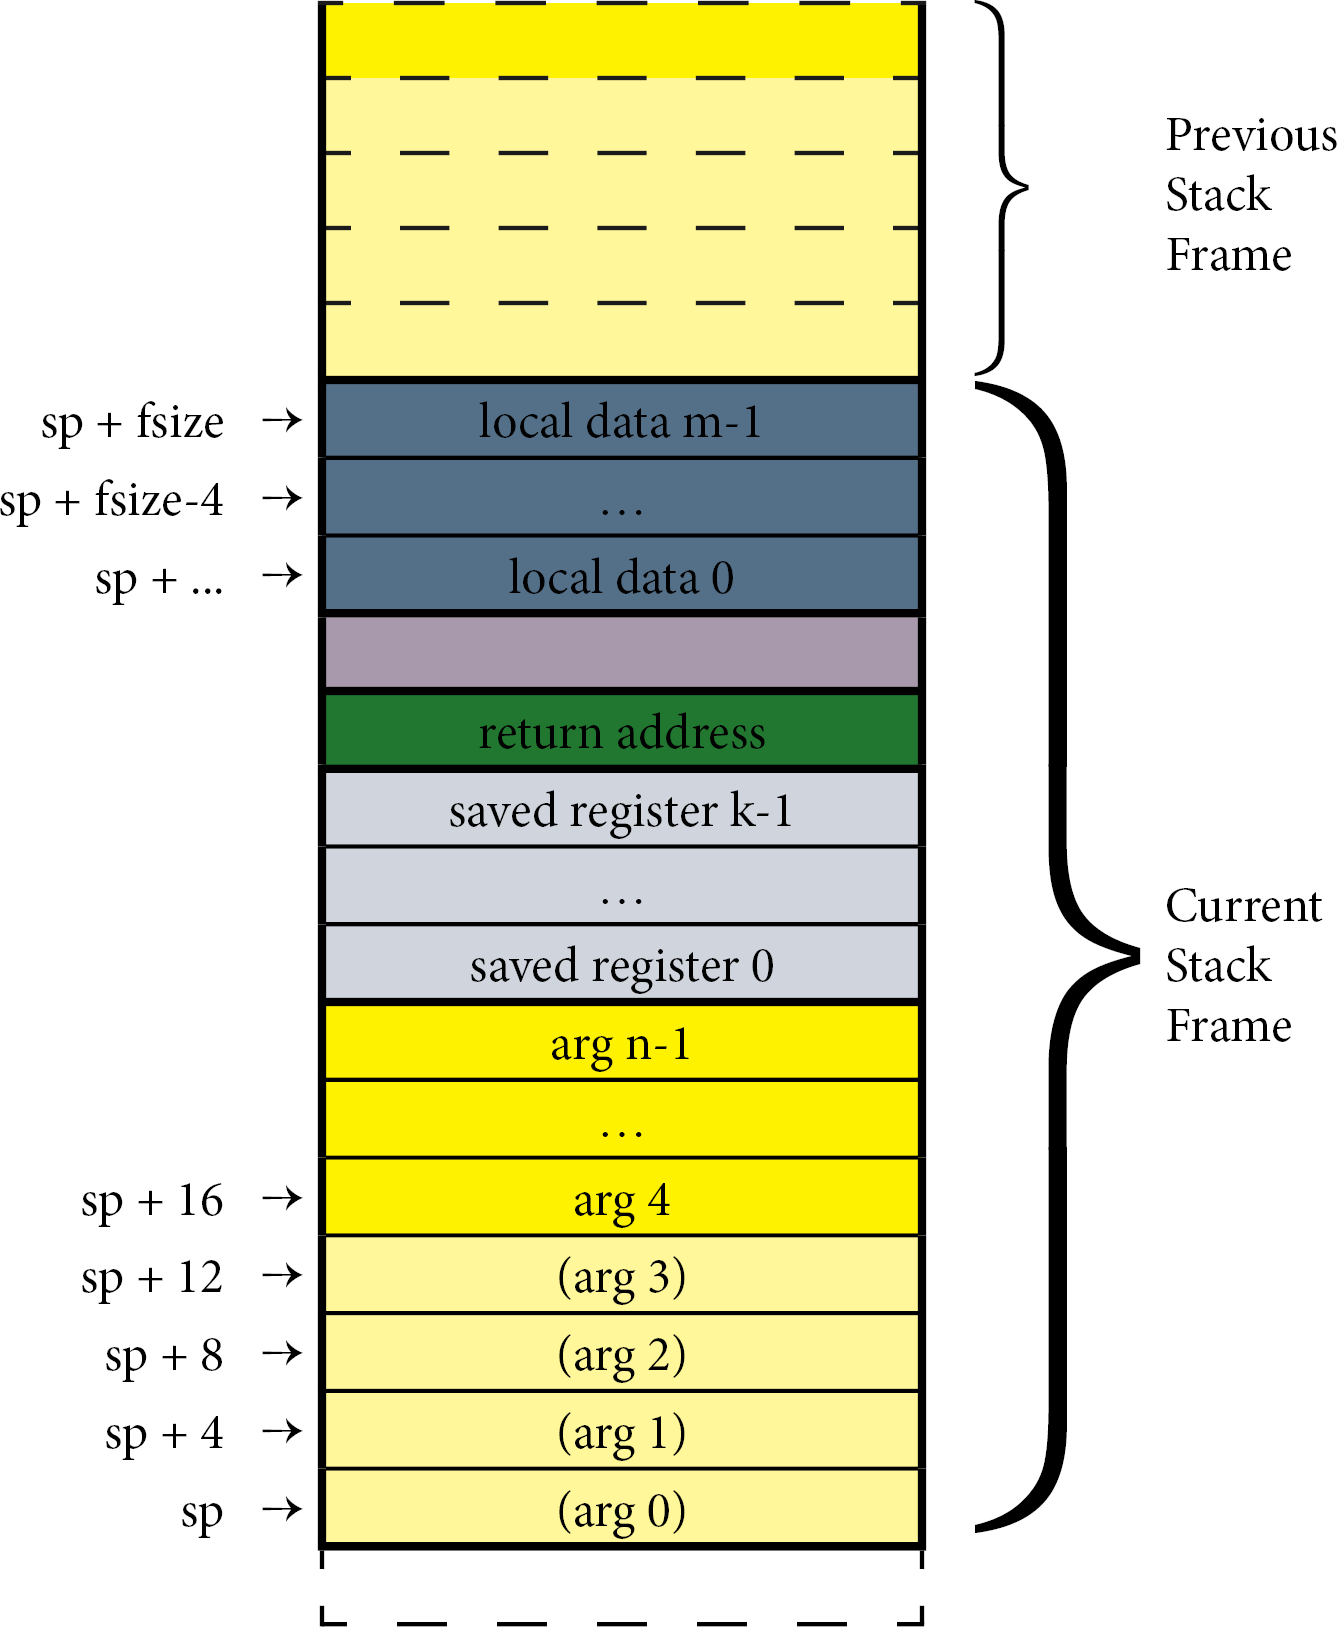
\includegraphics{stack-frame.png}
\caption{A MIPS stack frame}
\label{fig:stackframe}
\end{wrapfigure}

Notice that the stack frame has storage for all of the things we mentioned
     earlier. But as you may have realized not every procedure will need all
     these things. For example, a procedure may not require any argument space
     if it never makes a procedure call of its own (a so-called
     \textit{leaf-procedure}). Consider even a procedure that doesn't require
     any stack space (i.e. it doesn't need a stack frame at all). The rule of
     thumb to remember is that if something is omitted it shouldn't change the
     order of things listed in the generic stack frame specification. The
     omission simply has a size of zero.\\

The following subsections will give more specific information and examples on
     using the different parts of the stack frame.\\

\subsubsection{Return Address}

A procedure needs to remember the address of its caller so that it can
     return. When it is called this address is stored in the \texttt{\$ra}
     register. If a procedure makes a procedure call itself this value will be
     overwritten. Therefore we must save this value on our stack frame. Space
     for the return address is positioned below the local variable space. A
     procedure will commonly write the return address to the stack just after
     allocating its stack frame. Likewise it will restore the value of
     \texttt{\$ra} before unloading its stack frame. If the procedure does not
     make a procedure call itself, there is no need to save the return address
     to the stack.\\

Here is a quick example of saving/restoring the return address:
\begin{lstlisting}
proc:   addiu   $sp, $sp, -24   # 16 bytes for arguments + 8 bytes
        sw      $ra, 16($sp)    # store return address above arguments

        ...                     # do some stuff

        lw      $ra, 16($sp)    # restore return address
        addiu   $sp, $sp, 24    # pop off stack frame
        jr      $ra
\end{lstlisting}

\newpage
\subsubsection{Save Registers}
\label{sec:saveregs}

The calling convention allows certain registers (i.e. the save registers,
     \texttt{\$s0 .. \$s7}) to be saved to the stack by a procedure. A procedure
     only saves a save register if it intends to modify its value. In this way,
     we only go through the expense of saving a save register if we know its
     value is going to change locally within the procedure. Also note that it is
     the callee's responsibility to save registers, since it knows if it is
     going to modify them.\\

This process works similarly to how the return address register is saved to the
     stack. When the procedure is about to return, it needs to restore the
     original value of these registers. This way, the caller never is aware that
     they were modified (i.e. the entire process is transparent to the
     caller). A practical example that uses a save register is demonstrated in
     the next subsection.

\subsubsection{Arguments}

The most important thing to know about arguments in MIPS is that the four
     argument registers (\texttt{\$a0 .. \$a3}) are used to pass values to
     procedures. Of course, a procedure may require more than four arguments, in
     which case the stack is used to pass in the extra arguments.\\

A procedure's parameters are allocated by its caller and therefore exist in the
     caller's stack frame. The caller \textit{always} allocates space for the
     argument registers (i.e. 16 bytes), even if it passes fewer than four
     arguments. Furthermore it does not write any data into this space. It
     simply provides the callee with some space in case it needs to save the
     values of the argument registers. This is important if the procedure is
     going to invoke another procedure itself and need to overwrite the argument
     registers. Any more arguments are written directly to the stack by the
     caller.\\

To access parameters on the stack, we use positive offsets from the bottom of
     our stack frame. It is possible to use the stack frame register to refer to
     the bottom of our stack frame so that we just have to remember offsets from
     that point on\footnote{Interestingly I have seen some compilers use both
     the stack frame and stack pointer register to refer to the top of the
     stack. Also, some documentation on MIPS registers doesn't even specify a
     frame pointer register; instead, register \texttt{\$30} is another save
     register.}. Otherwise we can just use the stack pointer register to refer
     to everything, even when we have to push into the previous stack frame.\\

Here is a practical example. Consider the following C program that recursively
     computes the $N^{th}$ Fibonacci term (note that any system call wrappers
     implied by the source code denote direct system calls and not procedure
     calls):\\

\begin{lstlisting}[language=C]
int fib(int n)
{
    if (n <= 1)
        return n;
    return fib(n-1) + fib(n-2);
}

int main()
{
    print_integer(fib(read_integer()));
    print_character('\n');
    return 0;
}
\end{lstlisting}

Since we make two recursive calls that depend on parameter \texttt{n}, we will
     have to save the value of \texttt{n} on the stack so that we can recall it
     after making the first recursive call. We also have to save the return
     value of the first recursive call. We'll use the
     \hyperref[sec:saveregs]{save register} \texttt{\$s0} for this purpose.\\

Each call to \texttt{fib} will allocate 24 bytes on the stack since we must
     allocate at least 4 words for argument space plus some space for the return
     address (this procedure uses no local variables). The argument stack space
     will be used by \textit{both} the first and second recursive calls.\\

\lstinputlisting[title={{\lstname} - Computing a Fibonacci term}]{fib.s}

\newpage
\subsubsection{Local Variables}

Local variables are stack-allocated memory regions used while a procedure is
     executing and forgotten when a procedure returns. To access local variables
     within a procedure block, use offsets from the current value of the stack
     pointer register. These should be positive offsets that are multiples of 4
     bytes. Each local variable will have its own assigned offset from the stack
     pointer.\\

The stack frame diagram seen previously showed that local variables are stored
     toward the bottom of the stack frame (i.e. furthest away from the value of
     \texttt{\$sp}. Some compilers I've seen actually put this space between the
     argument space and the save register space. It really doesn't matter as
     long as you're consistent.\\

Consider the following C function (note that any system call wrappers implied by
     the source code denote direct system calls and not procedure calls). It
     prints out the integer ASCII values of an input string:\\

\begin{lstlisting}[language=C]
void foo()
{
    register int n, i;
    char buf[128];
    n = read_string(buf,sizeof(buf));
    for (i = 0;i < n;++i) {
        print_int(buf[i]);
        print_character(' ');
    }
    print_character('\n');
}
\end{lstlisting}

Note that this example is slightly non-trivial since we can't use a register to
     hold a text string buffer - we must allocate \texttt{buf} on the
     stack. Also recall that the C language reserved word \texttt{register} is a
     hint to the compiler not to allocate an object on the stack and instead
     optimize the value to a register. Since we are the compiler in this case,
     we will play nicely and respect the programmer's wishes. It's actually easy
     to use a register since the \texttt{int} data type corresponds to a single
     word that fits perfectly in a register.\\

The compiled code might look something like this:\\

\lstinputlisting{ascii.s}

Since \texttt{foo} is a simple leaf procedure, we only need to allocate space
     for the local variable \texttt{buf}. It turns out that our buffer size
     plays nicely with our stack pointer alignment requirement (8-byte
     boundaries). We would have to add in extra bytes to align to some multiple
     of eight. Note that it is up to you how to structure your local variable
     block. They do not necessarily need to align on any specific boundary
     though it may be beneficial to your implementation for you to do so.

\subsection{The Application Runtime}
\label{sec:runtime}

You may have heard the term \textit{runtime library}. On most platforms this
     refers to a small (or potentially large) segment of code inserted into your
     compiled program that provides runtime functionality. This library is
     unlike other libraries your program may have loaded as it provides core
     programming language functionality instead of some application-specific
     functionality. For example, the C language runtime performs initialization
     of global variables and calls \texttt{main}. It also takes the return value
     from \texttt{main} and passes it the system via \texttt{exit} to terminate
     the process. In more complex languages, the runtime library provides more
     support. For example, C++ provides runtime exception handling and dynamic
     type information.\\

When building a compiler for a language, you most likely will want to include
     some sort of minimal runtime support. For example, if you were wanting to
     define an application entry point (such as a \texttt{main} function) for
     your language, you probably want to include a minimal runtime that calls
     \texttt{main} and then calls \texttt{exit} with the return value from
     \texttt{main}. For example:

\begin{lstlisting}
    .text
    jal main
    move $a0, $v0
    li  $v0, 10
    syscall

    ... # compiled code goes here
\end{lstlisting}

If you are compiling a relatively unstructured language, then it is sufficient
     to simply inject a call to \texttt{exit} at the end of the program.

\section{Instruction Reference}
\label{sec:iref}

\end{document}
